\documentclass[12pt, a4paper]{report}

\usepackage{url}
\usepackage[utf8]{inputenc}
\usepackage{graphicx}
\usepackage{hyperref}
\usepackage{xurl}
\usepackage{textcomp}
\usepackage{float}
\usepackage{amsthm}
\usepackage{amssymb}
\usepackage{xcolor}
\usepackage{listings}
\lstset{language=Java,
    frame=lines,
    showspaces=false,
    showtabs=false,
    breaklines=true,
    showstringspaces=false,
    breakatwhitespace=true,
    commentstyle=\color{gray},
    keywordstyle=\color{blue},
    stringstyle=\color{red},
    basicstyle=\ttfamily,
    numbers=left,
    moredelim=[il][\textcolor{grey}]{$$},
    moredelim=[is][\textcolor{grey}]{\%\%}{\%\%}
}
\usepackage{adjustbox}

\usepackage[
    backend=biber,
    style=alphabetic,
    sorting=ynt
]{biblatex}
\addbibresource{darwinsquest.bib}

\newcommand*{\MyIncludeGraphics}[2][]{%
\begin{adjustbox}{max size={\textwidth}{\textheight}}
    \includegraphics[#1]{#2}%
\end{adjustbox}
}

\graphicspath{{img/}} % configuring the graphicx package globally

\theoremstyle{definition}
\newtheorem{exmp}{Example}[section]

\title{
    \begin{figure}[ht]
    \centering{}
    
\includegraphics[width=\textwidth]{logo} % remember best practice without extension, NO img/logo, img/logo.png or logo.png, but logo is enough
    \end{figure}
}
\author{
    Enrico Marchionni\\
    \texttt{enrico.marchionni@studio.unibo.it}
    \and
    Francesco Cipollone\\
    \texttt{francesco.cipollone@studio.unibo.it}
    \and
    Raffaele Marrazzo\\
    \texttt{raffaele.marrazzo@studio.unibo.it}
}
\date{\today}

\begin{document}

\maketitle

\begin{abstract}

    Darwin's Quest \cite{ontheoriginofspiecies} is a multi-level structured video game set in a post apocalyptic world,
    shaken by climate change. The goal is to survive natural selection by completing numerous battles,
    after choosing your genetically modified Banions\footnote{\emph{Banion}, meaning Battle Companion, is the monsters' name.}.

\end{abstract}

\tableofcontents

\chapter{Analysis}

\section{Requirements}

\subsubsection{Functional}

\begin{itemize}
    \item The player can choose between two game modes: Normal, Hard;
    \item At the beginning of the game, the player must be able to select four starter fight companions from a number of multiple choices;
    \item The game interface will consist of a board of levels in which the player moves. Each level will prompt a battle;
    \item The player's movement will be managed by tiles. Each tile is a battle tile.
        The movement will be determined by the use of a die. Said die value corresponds to the number of tiles that the player can move;
    \item The companions are able to evolve based on a linear evolution. Each time an evolution is triggered, the companions' statistics will increase;
    \item The player has to sequentially complete a series of levels, with increasing difficulty until meeting the final boss.
        The battles are engaged in 1v1 a turn-based combat fashion, with the ability to switch between companions or perform moves.
\end{itemize}

\subsubsection{Non-Functional}

\begin{itemize}
    \item The battle needs to be challenging for the player and will require a careful strategic plan planning ahead; \label{challengingbattle}
    \item The game performances must be acceptable;
    \item The game has to be portable and compatible with Windows, macOS, and Linux systems.
\end{itemize}

\section{Domain Model}

    The player can move inside the board map bounds. The map contains the player, the enemies, and battle tiles.
    Landing on this tile will prompt the beginning of a battle and losing the fight will trigger the game over.

    The player owns four Banions. Each Banion has an intrinsic elemental type, such as fire, water, grass, rock, air, electro,
    and is associated has a set of moves, which are divided into groups based on the Banions' elemental type. A certain Banion with a certain
    type only retains moves of its same elemental type plus neutral moves, e.g. A fire Banion can only use fire moves and neutral moves,
    and cannot perform other types' moves.

    Banions in our game are the following:

\begin{table}[ht]
    \begin{center}
    \begin{tabular}{| c | c | c | c | c | c | c |}
        \hline
        Banion & Element \\ [0.5ex] % Fire & Water & Grass & Rock & Air & Electro
        \hline\hline
        Hefty & Air \\
        \hline
        Aotori & Air \\
        \hline
        Buzzwings & Air \\
        \hline
        Jolbat & Electro \\
        \hline
        Sparkleap & Electro \\
        \hline
        Zapameleon & Electro \\
        \hline
        Infernhog & Fire \\
        \hline
        Blazechick & Fire \\
        \hline
        Scorchspore & Fire \\
        \hline
        Florastump & Grass \\
        \hline
        Herbroot & Grass \\
        \hline
        Flingleaf & Grass \\
        \hline
        Stonemaul & Rock \\
        \hline
        Spebble & Rock \\
        \hline
        Stonohorn & Rock \\
        \hline
        Aquamuck & Water \\
        \hline
        Hydrashell & Water \\
        \hline
        Quacktide & Water \\
        \hline
    \end{tabular}
    \caption{\label{table:banions} Banions}
    \end{center}
\end{table}

    The available moves for the Banions are:

\begin{table}[H]
    \begin{center}
    \begin{tabular}{| c | c | c |}
        \hline
        Move & Element & Damage \\
        \hline \hline
        Tornado & Air & 3 \\
        \hline
        Aero Blast & Air & 3 \\
        \hline
        Breeze & Air & 3 \\
        \hline
        Monsoon & Air & 4 \\
        \hline
        Aero Slash & Air & 4 \\
        \hline
        Spark & Electro & 3 \\
        \hline
        Lightning & Electro & 3 \\
        \hline
        Thunderbolt & Electro & 3 \\
        \hline
        Volt Blitz & Electro & 4 \\
        \hline
        Surge Wave & Electro & 4 \\
        \hline
        Fireball & Fire & 3 \\
        \hline
        Flame & Fire & 3 \\
        \hline
        Torch & Fire & 3 \\
        \hline
        Magma Burst & Fire & 4 \\
        \hline
        Brazier & Fire & 4 \\
        \hline
        Meadow & Grass & 3 \\
        \hline
        Foliage Strike & Grass & 3 \\
        \hline
        Seed Barrage & Grass & 3 \\
        \hline
        Verdant Beam & Grass & 4 \\
        \hline
        Spores & Grass & 4 \\
        \hline
        Earthquake & Rock & 3 \\
        \hline
        Landslide & Rock & 3 \\
        \hline
        Bedrock Bash & Rock & 3 \\
        \hline
        Boulder Burst & Rock & 4 \\
        \hline
        Pebble Pummel & Rock & 4 \\
        \hline
        Tsunami & Water & 3 \\
        \hline
        Whirlpool & Water & 3 \\
        \hline
        Aqua Blast & Water & 3 \\
        \hline
        Coral Spear & Water & 4 \\
        \hline
        Waterfall & Water & 4 \\
        \hline
    \end{tabular}
    \caption{\label{table:moves} Moves}
    \end{center}
\end{table}

    \pagebreak
    Some Banions will also have neutral-type moves:

\begin{table}[H]
    \begin{center}
    \begin{tabular}{| c | c | c |}
        \hline
        Move & Element & Damage \\
        \hline \hline
        Claw & Neutral & 2 \\
        \hline
        Roar & Neutral & 2 \\
        \hline
        Bite & Neutral & 2 \\
        \hline
        Impale & Neutral & 2 \\
        \hline
        Kick & Neutral & 2 \\
        \hline
        Strike & Neutral & 2 \\
        \hline
        Blast & Neutral & 2 \\
        \hline
        Slash & Neutral & 2 \\
        \hline
        Swipe & Neutral & 2 \\
        \hline
        Pulse & Neutral & 2 \\
        \hline
        Beam & Neutral & 2 \\
        \hline
        Slam & Neutral & 2 \\
        \hline
        Hurl & Neutral & 2 \\
        \hline
        Punch & Neutral & 2 \\
        \hline
        Poke & Neutral & 2 \\
        \hline
    \end{tabular}
    \caption{\label{table:neutralMoves} Neutral Moves}
    \end{center}
\end{table}

    Elemental reactions, that are bounded to moves, are defined as follows:

\begin{table}[ht]
    \begin{center}
    \begin{tabular}{| c || c | c | c | c | c | c |}
        \hline
        Player \textbackslash Enemy & Air & Electro & Fire & Grass & Rock & Water \\ [0.5ex]
        \hline\hline
        Air         & - & * & * & - & + & + \\
        \hline
        Electro     & * & + & * & - & * & * \\
        \hline
        Fire        & * & * & * & + & * & - \\
        \hline
        Grass       & + & + & - & * & - & * \\
        \hline
        Rock        & - & * & * & + & * & * \\
        \hline
        Water       & - & * & + & * & * & * \\
        \hline
    \end{tabular}
    \caption{\label{table:elements} Elements}
    \end{center}
\end{table}

    \textit{Each companion in the game will have a personal set of statistics, such as attack (ATK), defense (DEF), health points (HP).
    The values make up the base statistics of a certain companion.}

    In every level, there are two player entities: the player and the opponent (NPC\footnote{\textbf{NPC: Non-Playable Character}}). These entities deploy their companions, which will fight 1v1.
    A level consists of a battle phase, and leveling phase:
\begin{itemize}
    \item \textbf{Battle phase}: during the player's fight turn, it is possible to switch their active companion to a different one, 
        or the player can perform a move. Upon the player's active companion's defeat, they will be forced to switch to another one. 
        If the player is out of eligible companions the fight is over.
    \item \textbf{Leveling phase}: upon the player's victory, Experience Points will be assigned to the Banions. If a Banion obtains enough XP\footnote{\textbf{XP}: Experience Points} it will evolve.
\end{itemize}

    The fight mechanics are considered a project challenge for their complexity \ref{challengingbattle}, from the elemental reaction logic to the moves' management.

    \begin{figure}[H]
    \centering{}
    \caption{Model UML}
    \MyIncludeGraphics{model}
    \end{figure}

\chapter{Design}

\section{Architecture}

    This project is developed in \href{https://en.wikipedia.org/wiki/Model%E2%80%93view%E2%80%93controller}{MVC} (Model, View and Controller) architecture.
    In our architecture the \textbf{Controller} is the entry point of the application. It instantiates the \textbf{View} that instantiates the \textbf{Controller} itself.
    The latter represents the main class, and it coordinates the interaction between the \textbf{View} and the \textbf{Model}, which is instantiated at a proper time by
    the \textbf{Controller}, following the MVC architectural pattern.

    In our architecture the main classes are \textbf{JavaFXView} (View), \textbf{ControllerImpl} (Controller) and \textbf{EngineImpl} (Model). The
    first one is responsible for the collection of input and shows the output, the third one contains game main components and the second one is the link between them.

    \begin{figure}[ht]
    \centering{}
    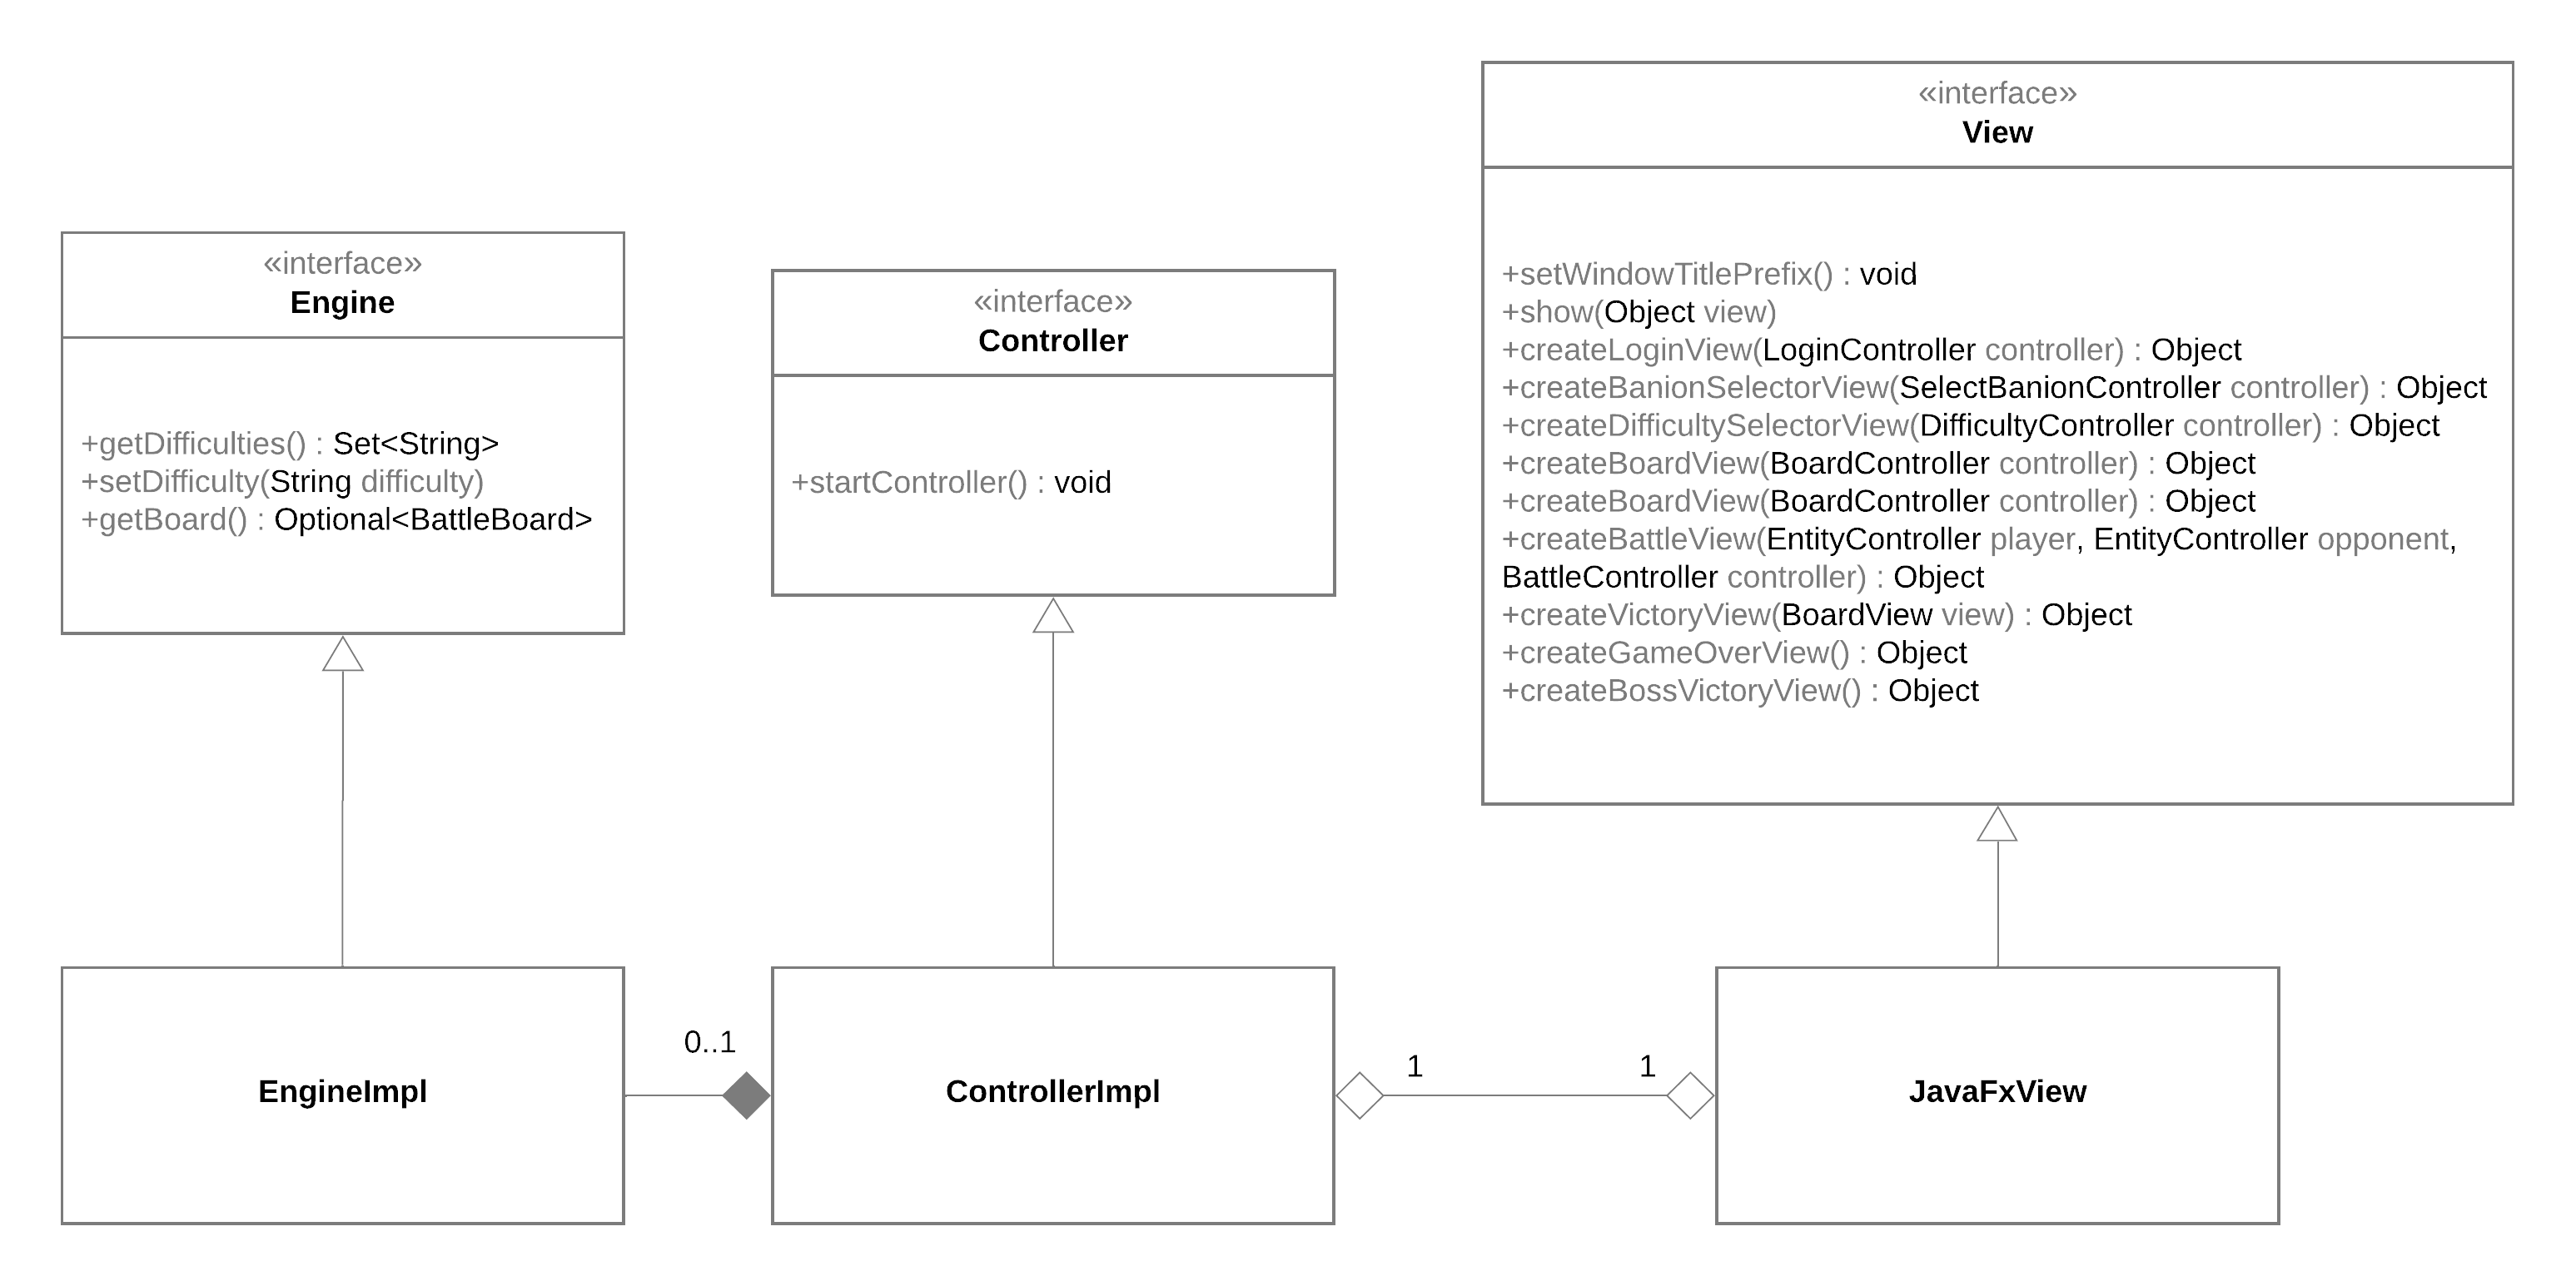
\includegraphics[width=12cm]{MVC_main_classes}
    \caption{UML Model-View-Controller}
    \end{figure}

\section{Details}

    \subsection*{Enrico Marchionni}

        \subsubsection{Game Difficulty}

            \paragraph{Problem}
            
            Giving the possibility to choose between different thought games.
            Each difficulty should determine for example the number of tiles for the \emph{Board}, the moving \emph{Strategy} in it,
            the number and \emph{Element} of the \emph{Opponent}'s \emph{Banion}s, the \emph{AI} for each \emph{Opponent}...
            A requirement is that this problem has to be resolved in an extendible way.
            So once the system is built, adding a difficulty must be easy and fast according to \emph{OCP} (open closed principle).

            \paragraph{Solution}

            The element \emph{Board} is the main entity of this game because it determines how much
            levels have to be completed to win the game. So the main \emph{Model} class that is responsible for
            the difficulties is the \emph{Engine} class. It retrieves the \emph{Board} and everything else go by itself
            only by selecting the \emph{Difficulty}. The difficulty has the goal to decide the \emph{Board} \emph{Strategy} of
            movement, the number of levels and the \emph{AI} associated with the \emph{Opponent}. Each \emph{Opponent} will
            be created by the \emph{Board} at the right moment through an \emph{OpponentFactory} that was created by the \emph{Difficulty}
            itself.

            \begin{figure}[ht]
            \centering{}
            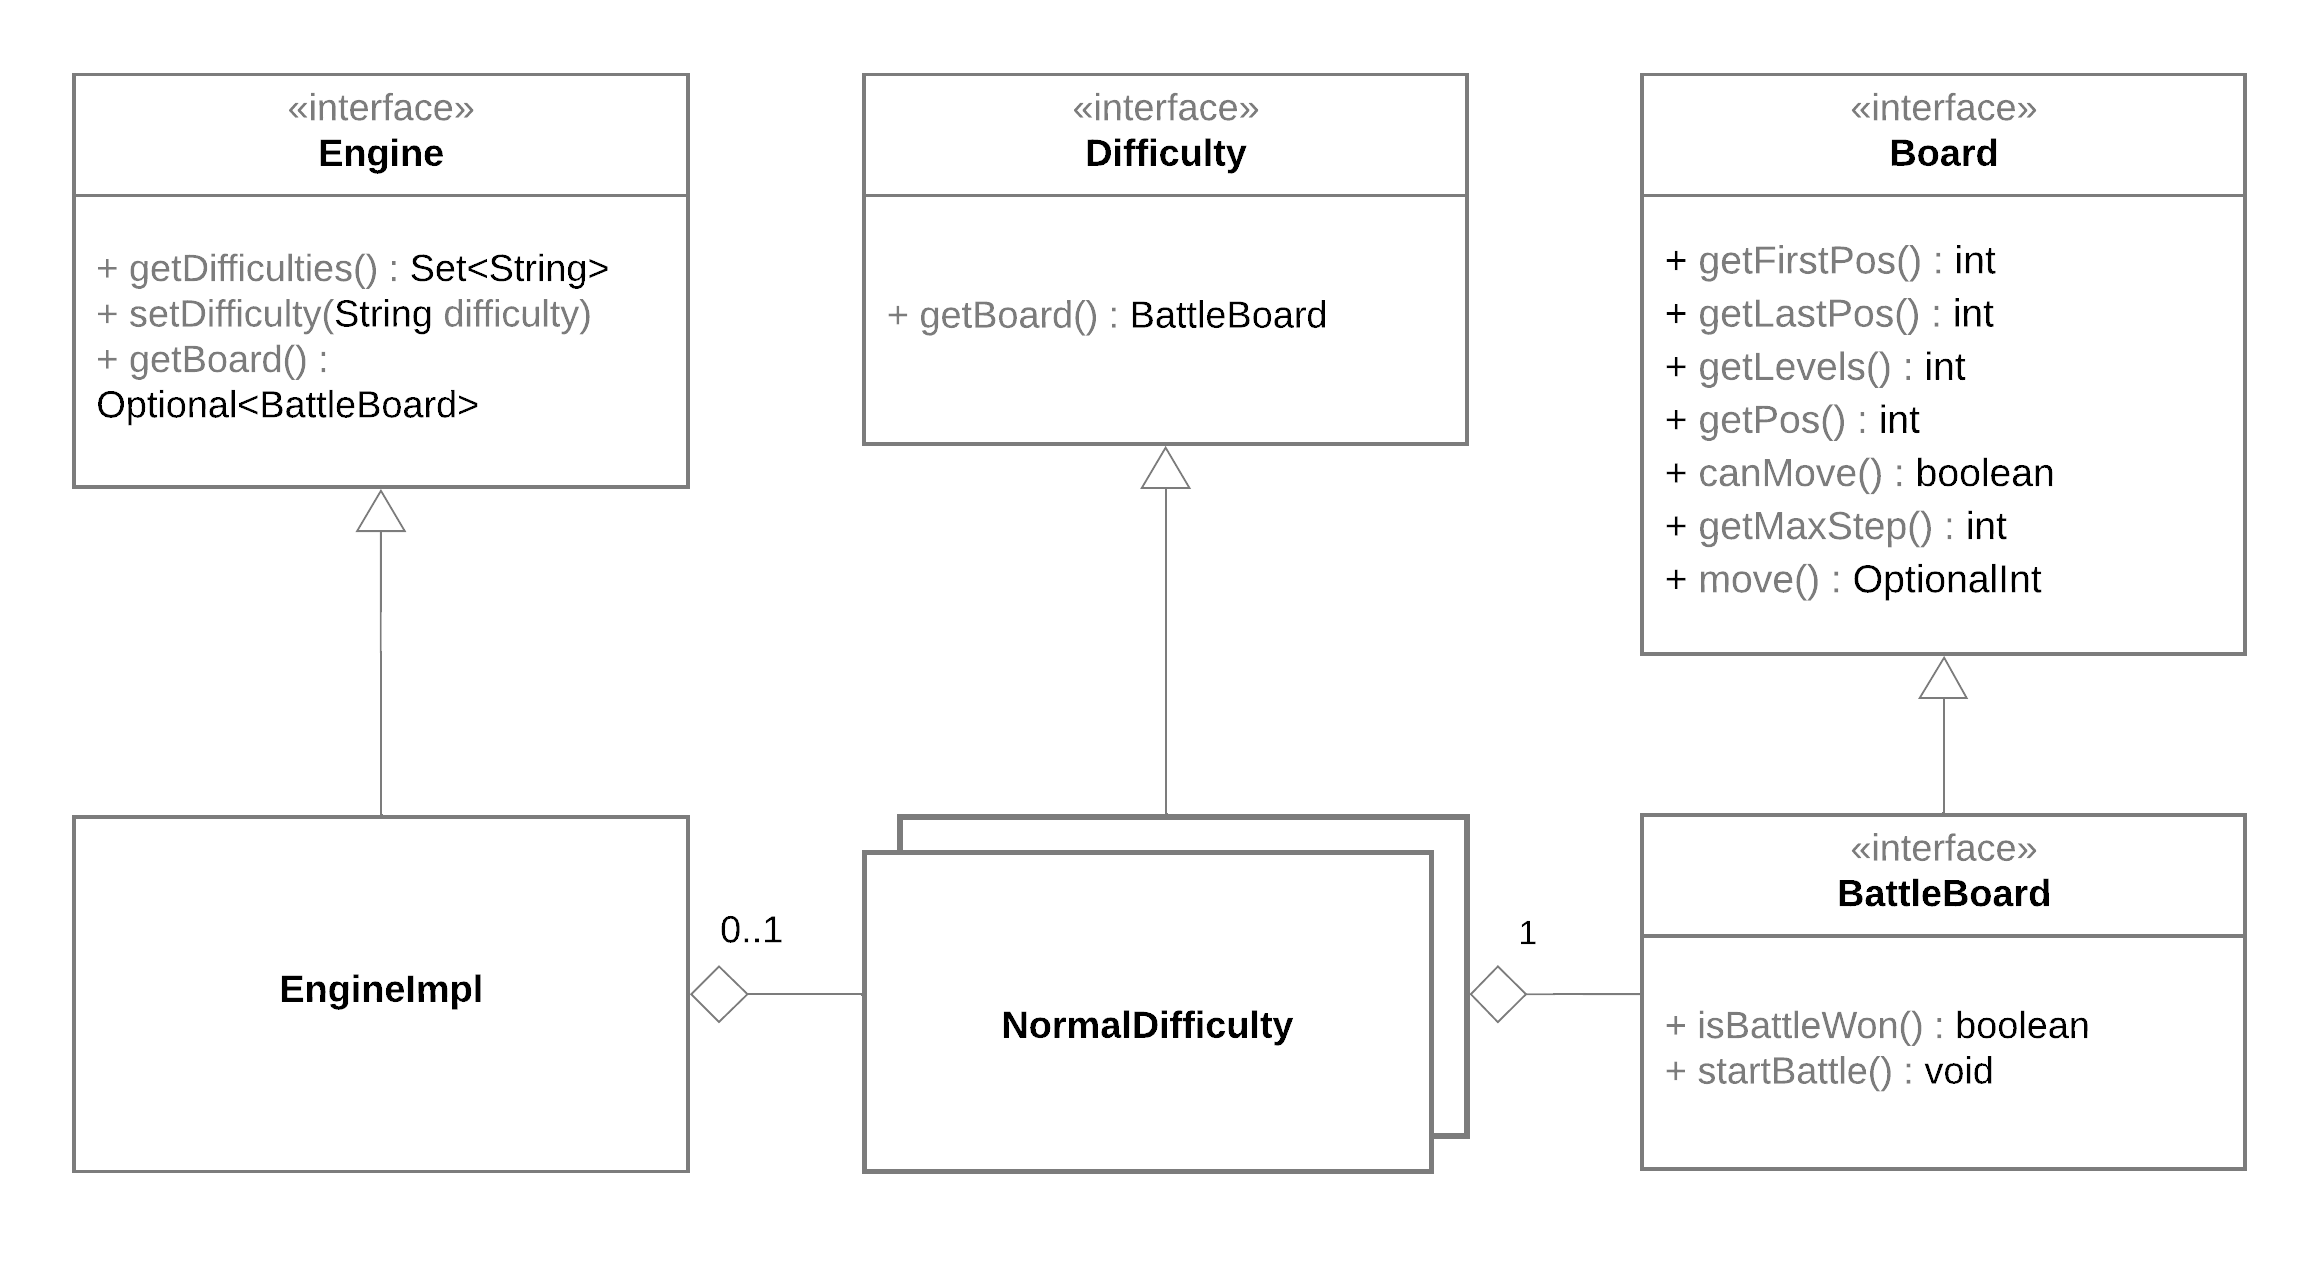
\includegraphics[width=\textwidth]{difficulty}
            \caption{UML difficulty}
            % \label{img:difficulty}
            % \ref{img:difficulty}
            \end{figure}

            \paragraph{Pattern}

            The \emph{Difficulty} decides the \emph{Board} step of movement by passing a \emph{PositiveIntSupplier} to \emph{Board} constructor via \emph{Strategy}.
            Furthermore the \emph{Difficulty} decides also the \emph{OpponentFactory} implementation to pass to the \emph{Board} via \emph{Strategy}.
            The \emph{OpponentFactory} can be considered as \emph{Abstract Factory} because every single implementation of \emph{Difficulty} could pass
            a different implementation of \emph{OpponentFactory} to the relative \emph{BattleBoard}.
            
        \pagebreak

        \subsubsection{\emph{Banion identification}}

            \paragraph{Problem}

            We wanted to make two \emph{Banion}s with same name and statistics be considered different at \emph{Domain Model} level.

            \paragraph{Solution}

            After evaluating different options such as not overriding \emph{Banion}'s equals, we decided to use
            \href{https://docs.oracle.com/en/java/javase/17/docs/api/java.base/java/util/UUID.html}{\textit{java.util.UUID}} class to identify every single \emph{Banion} instance.
            In this way it is possible for a player for example to have in the inventory two \emph{Banion}s with the same name twice, because they are different.
            
        \pagebreak

        \subsubsection{\emph{Banion modified}}

            \paragraph{Problem}

            In the \emph{View} each \emph{Banion} represented could be modified and should be seen always in most updated state.
            Furthermore potentially there could be more that one \emph{View} representing the same \emph{Banion}.

            \paragraph{Solution}

            I decided to make the Banion observable for its changed state.

            \begin{figure}[ht]
            \centering{}
            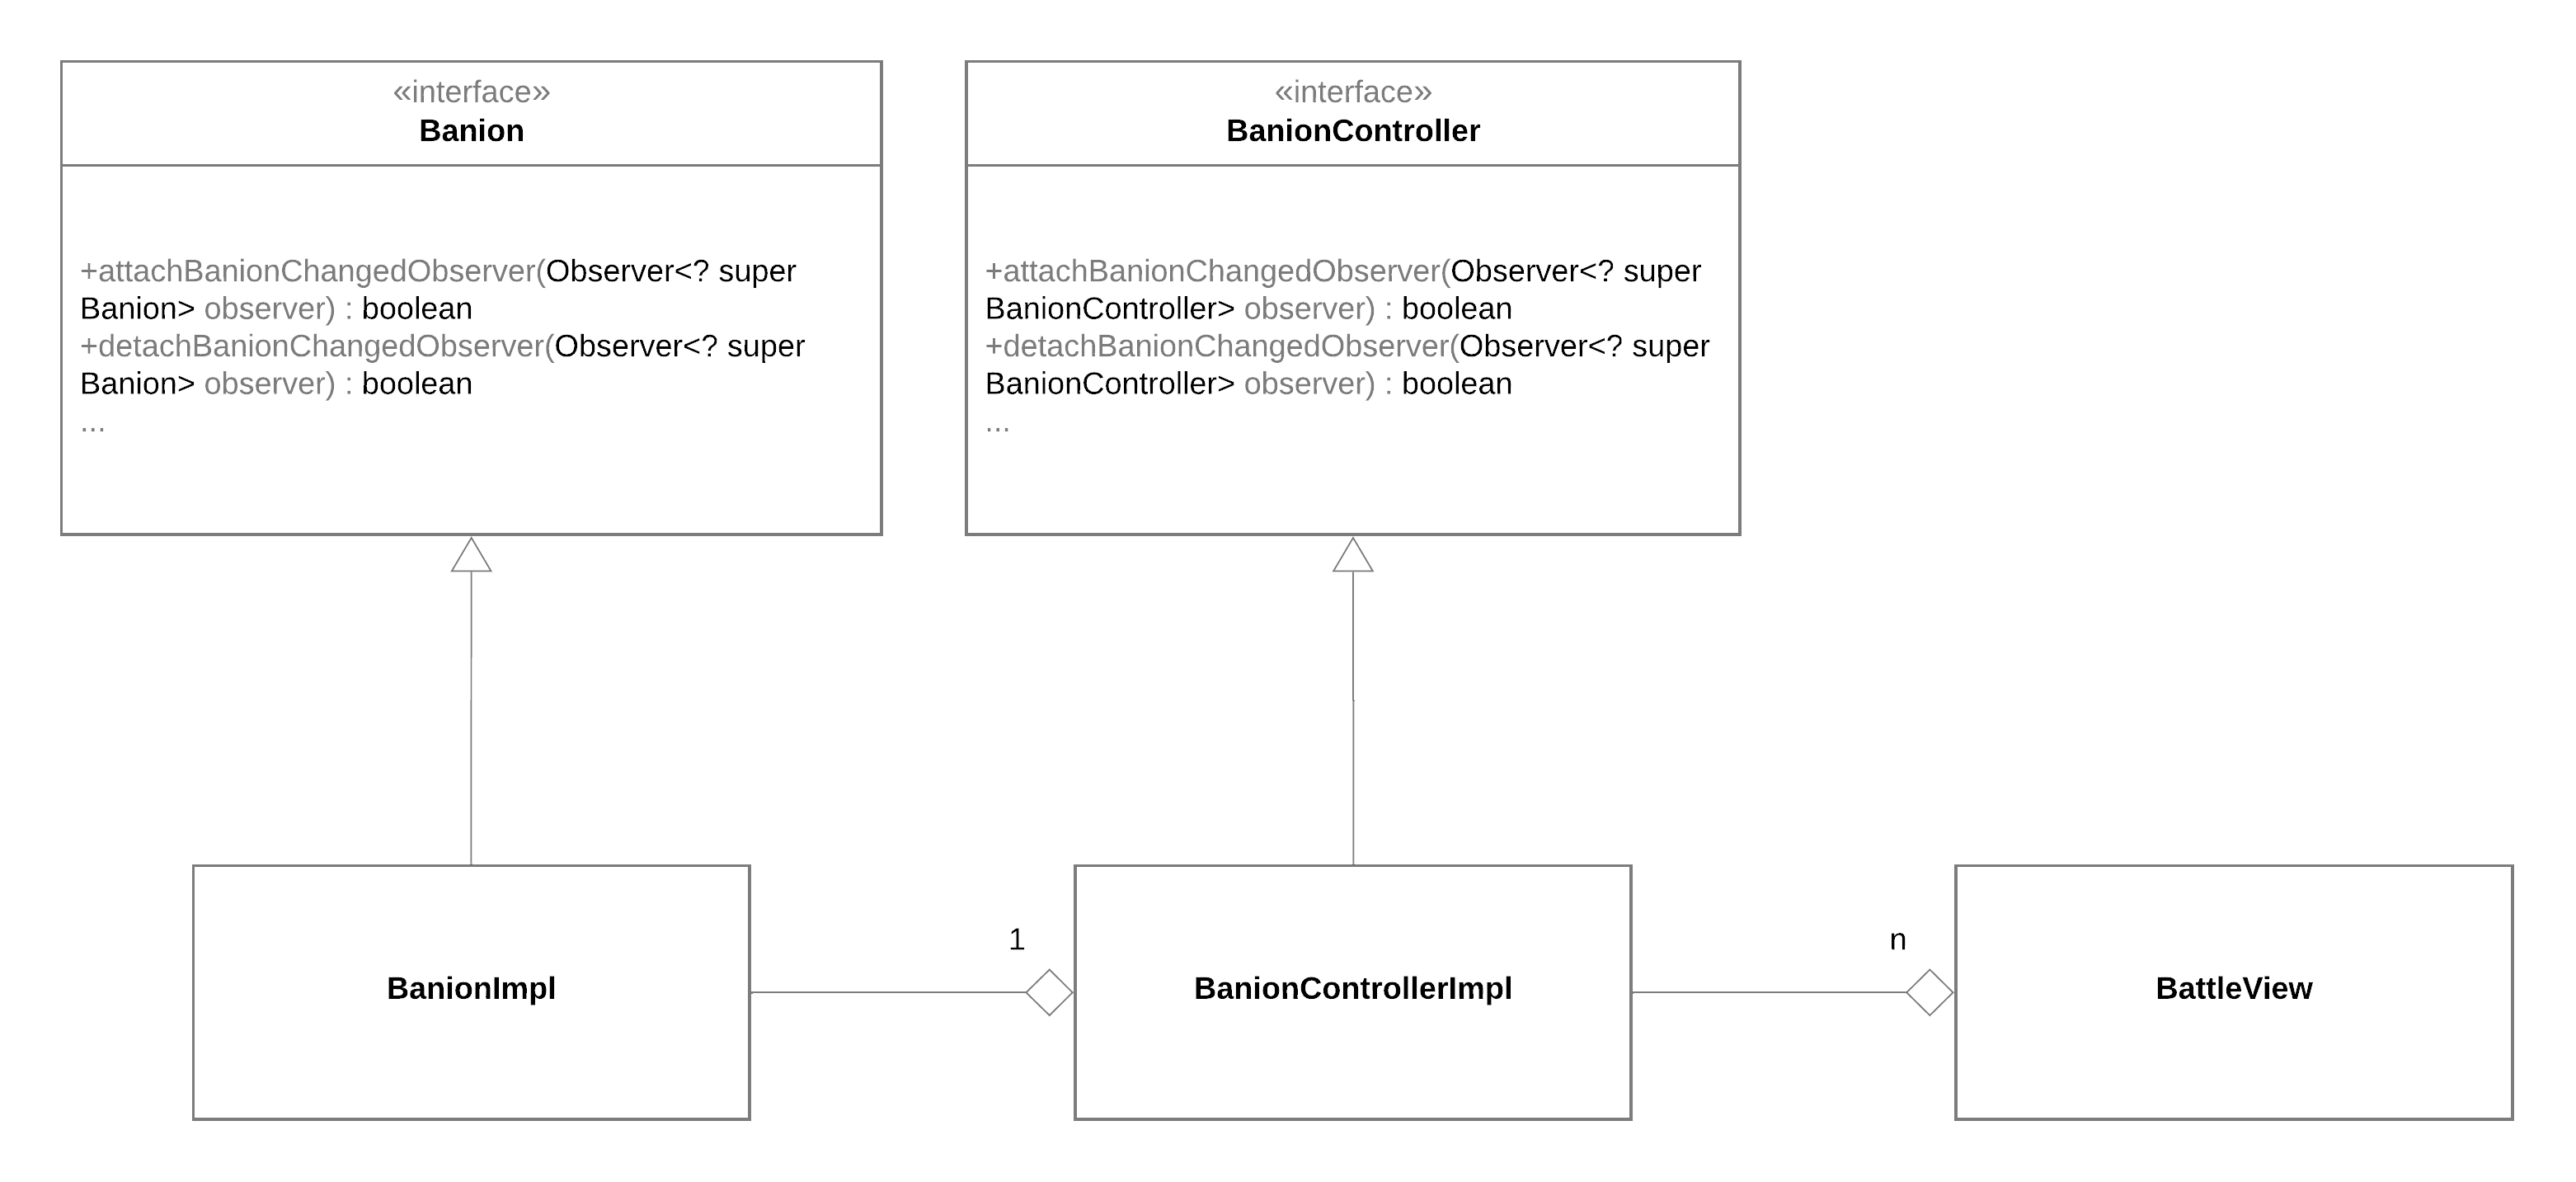
\includegraphics[width=\textwidth]{banion_changed}
            \caption{UML Banion Observer}
            \end{figure}

            \paragraph{Pattern}

            The \emph{Observer} pattern was adopted to notify changes of state from the specific \emph{Banion}.
            \emph{BanionImpl} is the subject (the observable object) while \emph{BanionControllerImpl} and then \emph{BattleView} are the Observers.
            In specific \emph{BanionImpl} is observed from \emph{BanionControllerImpl} while \emph{BanionControllerImpl} is observed from \emph{BattleView}.
            \emph{BanionControllerImpl} is a "read only" \emph{Banion} wrapper that decouples \emph{Model} from \emph{View}.
            
        \pagebreak

        \subsubsection{\emph{Element}s, \emph{Move}s and \emph{Banion}s Generation}

            \paragraph{Problem}
            
            Generating game entities: \emph{Element}, \emph{Move} and \emph{Banion}. Our game needs a consistent number of \emph{Banion}s \ref{table:banions} to be playable.
            It would better if they could be the same every time the application starts: same names, same sprites, same moves...
            Independently from the user progresses it would be nice for a user to choose between the same set of Banions at the beginning of every new the game.

            \paragraph{Solution}

            The problem is that somehow these entities has to be created, so how I decided to do that is the solution.
            At the beginning I started from the generation of \emph{Element}s \ref{table:elements} by coding each one in Java classes.
            The two main problems I observed were the expansion of classes and the inability to easily and quickly add new ones.
            After that I took time to think at a more extendible and cleaner solution, at the end I decided to go for the deserialization.
            I decided to create in the MVC \emph{Controller} a system to deserialize entities from file.
            In specific I chose \textit{.json}, using \href{https://github.com/google/gson}{Google Gson} library.
            
            I also wanted to make sure to avoid duplication of information.
            We decided that every single entity must be identifiable by name.
            So I created three files, one for each entity to generate, following this structure:
            \begin{itemize}
                \item \emph{Element} \textrightarrow independent from the other entities;
                \item \emph{Move} \textrightarrow dependent from \emph{Element} entities (each \emph{Move} is associated with one \emph{Element});
                \item \emph{Banion} \textrightarrow dependent from \emph{Element} and \emph{Move} entities (each \emph{Banion} is associated with one \emph{Element} and 4 \emph{Move}s);
            \end{itemize}

            I also decoupled file reading from entities generation.
            I put in the \textit{darwinsquest.config} package classes to read from file while in \textit{darwinsquest.config} I put the Factories according to \emph{SRP} (single responsibility principle).

            \paragraph{Pattern}

            The entities are created by using \emph{Abstract Factory} pattern.
            \emph{ElementFactory}, \emph{MoveFactory} and \emph{BanionFactory} retrieves the deserialized data with the shape of a set.

            \paragraph{Comments}

            Following this scheme in future it could be easily add the functionality of writing a system to save user progress.
            This would consist essentially on storing user \emph{Banion}s data in a folder (ex. \emph{.darwinsquest} in the user folder) and reload them after the login operation.
            For what concerns \emph{User} and \emph{Board} progresses serialization it should be thought in organization, and it would be integrated with the serialization/deserialization of entities.

        \pagebreak

        \subsubsection{\emph{Board Opponents}}

            \paragraph{Problem}

            How to represent \emph{BattleTile}s in the \emph{Board}, and when to create \emph{Opponents} for each level.

            \paragraph{Solution}

            The \emph{BattleBoard} is a specific board that contains the concepts of battle and levels.
            Each movement in the \emph{Board} brings the player over a new \emph{BattleTile}.
            The \emph{BattleBoard} was specifically created by the selected \emph{Difficulty} with a particular \emph{OpponentsFactory} implementation.
            Once the player is to start a battle its specific opponent is created at that moment.

            \begin{figure}[ht]
            \centering{}
            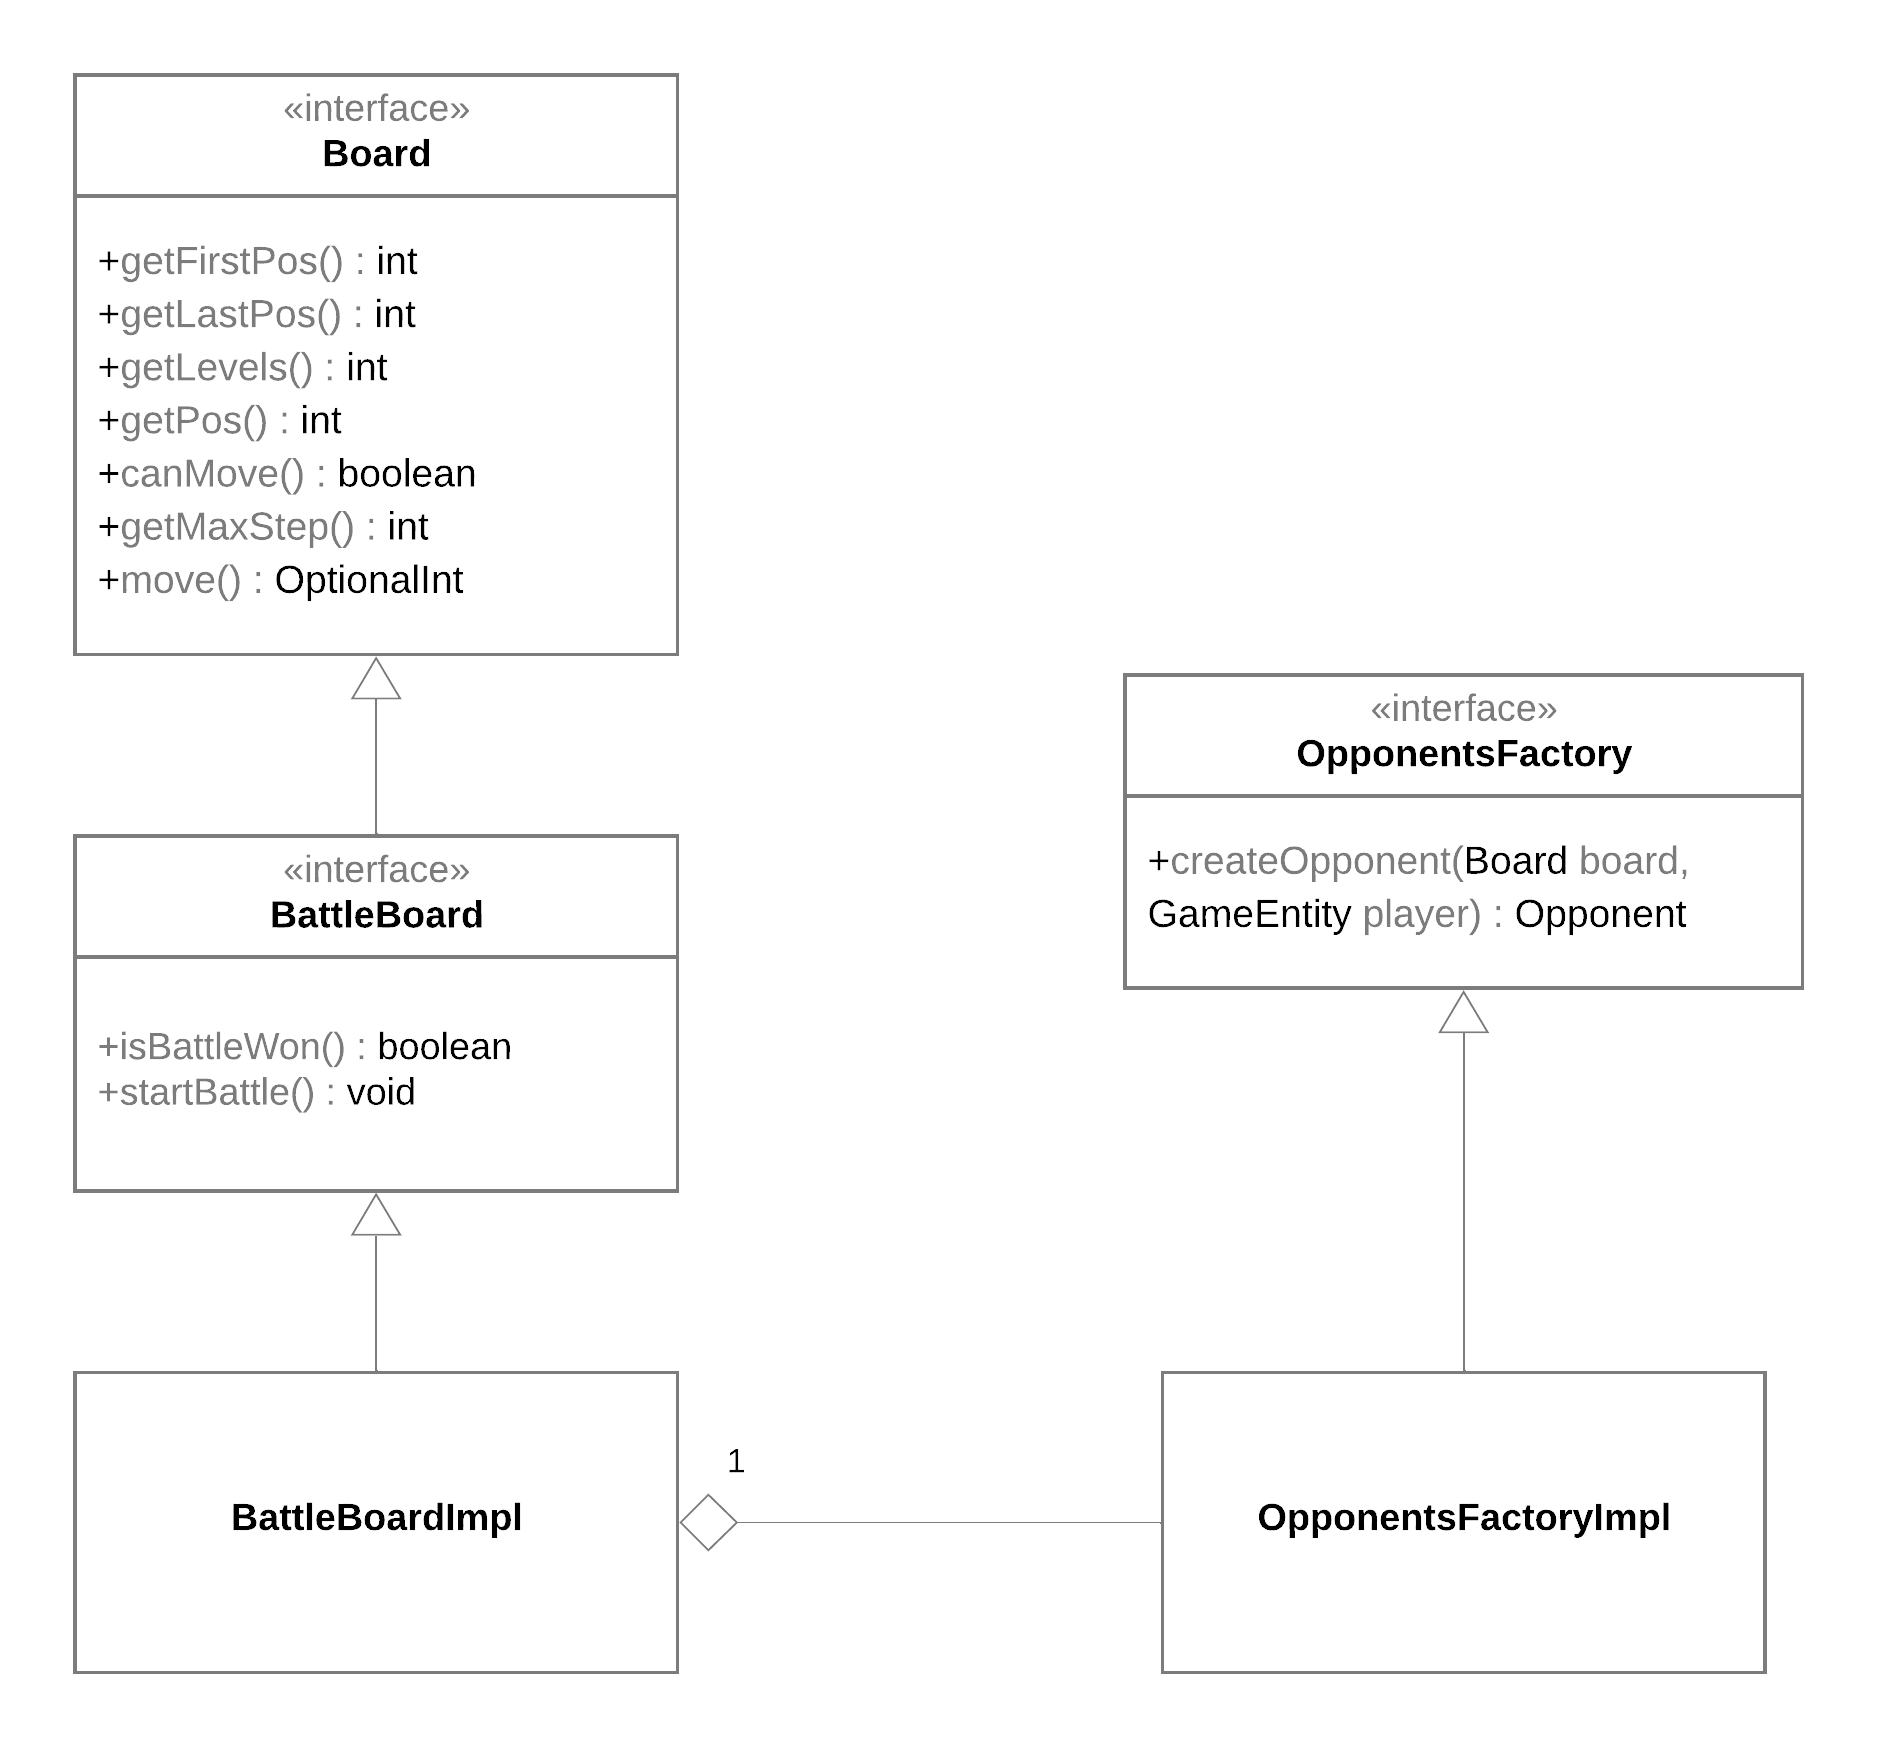
\includegraphics[width=\textwidth]{opponents_creation}
            \caption{UML Board Opponents}
            \end{figure}

            \paragraph{Pattern}

            The \emph{OpponentsFactory} is passed via\emph{Strategy} at the specific \emph{BattleBoard}.
            
        \pagebreak

        \subsubsection{\emph{Sprite}s}

            \paragraph{Problem}

            Each \emph{Banion} should be represented by a \emph{Sprite} in the \emph{View}.

            \paragraph{Solution}

            I considered that each \emph{Banion} is uniquely identified by its name.
            So I decided to put the necessary data in the same \textit{.json} file that contained also the \emph{Banion}s information.
            By doing that I created a \emph{BanionsSpriteFactory} class in the \emph{View} that has to read \emph{Sprite} record (it contains \emph{Banion} .png information).
            Each banion will be associated in the \emph{View} to its \emph{Sprite} by its name (this can be seen in \emph{ChooseBanionMenuView} constructor).
            
        \pagebreak

        \subsubsection{View}

            \paragraph{Problem}

            How to separate concerns in the chosen \emph{JavaFX} library in MVC.
            How to decouple style from showing controls, for example how to specify each \emph{Scene} font in a \emph{DRY} (don't repeat yourself) way.

            \paragraph{Solution}

            I started by using \textit{.css} files to specify style and \textit{.fxml} to specify layouts for each Container.
            I created a Controller for each Container.
            I created a \textit{View} interface that is a generic interface with the aim to create and show different views.
            In this way the \textit{View} interface remains generic and could potentially change without modifying its interfaces.
            
        \pagebreak

    \pagebreak

    \subsection*{Francesco Cipollone}

    \subsubsection{\underline{Game Entity - Player \& Opponent}}
    \paragraph{Problem}
    A player and opponent need to be generalised into a broader concept, such as a game entity.
    \paragraph{Solution}
    The interface \verb|GameEntity| was created to represent both the player entity and the opponent entity.
    It extends \verb|GameObject|, which represents the fundamental entities of the game.\\
    To encapsulate all the common aspects of any game entity an abstract class called \verb|AbstractGameEntity| was created. Its main purpose is to handle the inventory, leaving all the
    entity decisions (such as deploying a Banion, selecting a move, swapping a Banion, etc.) to the concrete entities.\\
    The \verb|Player| and \verb|Opponent| can now handle those decisions with the input and the AI respectively.
    In \verb|PlayerImpl| specifically, a static boolean method was added to check the validity of a username, by using a \textit{regular expression}.
    A valid username is defined by these guidelines:

    \begin{itemize}
        \item A nickname must:
        \begin{itemize}
            \item Not be \verb|null| nor blank;
            \item Start with an alphabetical character;
            \item Not start with one or more digits;
            \item Not start nor end with one or more symbols;
            \item Not start nor end with one or more underscores;
            \item Not include any white spaces;
            \item Not include Unicode characters.
        \end{itemize}
        \item A nickname may include:
        \begin{itemize}
            \item One or more underscores between the first and last characters;
            \item Digits after the first character.
        \end{itemize}
    \end{itemize}

    \begin{exmp}
        Nickname examples:
        \begin{itemize}
            \item[\checkmark] \textbf{Valid}: \verb|Alice_hash7|, \verb|Bob|
            \item[$\times$] \textbf{Invalid}: \verb|!Alice|, \verb|Amélie|
        \end{itemize}
    \end{exmp}

    The game entities make use of an observer to notify when they decided to swap a Banion during a battle.

    \begin{figure}[H]
    \centering{}
    \caption{GameEntity UML diagram.}
    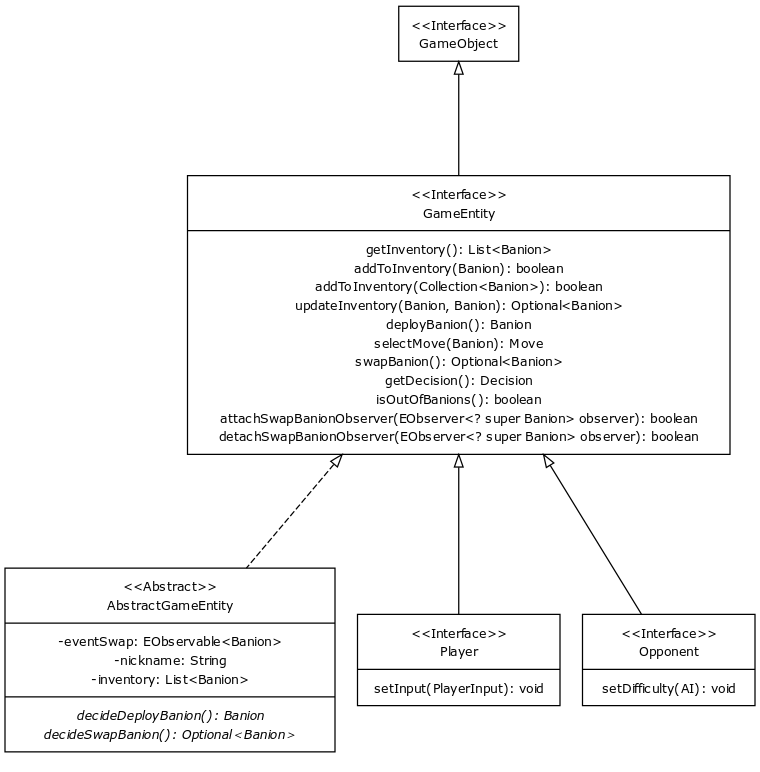
\includegraphics[width=\textwidth]{game_entity_uml}
    \end{figure}

    \subsubsection{\underline{Inventory}}
    \paragraph{Problem}
    Every game entity needs to possess an inventory to store their Banions.
    \paragraph{Solution}
    We firstly conceived the inventory to be an object that could hold both Banions and other items, however since the items were scrapped for the lack of time,
    the concept of the inventory regressed to a simple list held in each game entity instance.\\
    The inventory permits add and update operations. The latter removes a given Banion in favour of another one.\\
    A crucial characteristic of the inventory is that it does not allow the insertion of a Banion that is already present. Specifically, it checks equality on the
    Banion's UUID: Banions that are \textit{alike} are allowed, \textit{identical} ones are not.

    \subsubsection{\underline{Evolution}}
    \paragraph{Problem}
    Each Banion must be able to evolve by gaining experience points and boosting its statistics.
    \paragraph{Solution}
    An \verb|Evolvable| interface is introduced: this interface contains the methods signatures that allows Banions to evolve.\\
    To prompt an evolution, the Banion class has to use an \verb|Evolution|.
    The \verb|Evolution| interface, which can also be implemented functionally, allows the given Banion to evolve, while basing said evolution
    on a given condition.\\
    While the use of a \verb|Predicate<Banion>| does not affect the Player's Banions, which are evolved by an experience points system\footnote{An evolution
    is prompted when the maximum XP value is reached. The current XP will be reset to zero, or to any exceeding amount left from reaching said ceiling.},
    it allows a diverse and customizable evolution for the Opponent's Banions by permitting different evolution approaches.\\
    The \verb|Evolution| interface allows the creation of different kind of evolutions, such as tree evolutions, linear evolutions, etc.\\
    This version uses a \verb|LinearEvolution|, meaning that the player cannot choose what and how to evolve their Banions: each statistics will be
    jointly evolved.\\
    The aforementioned approach additionally incorporates a maximum hp ceiling, which means that if the current hp statistic reaches the maximum allowable value,
    further evolutions will not increase said statistic.

    \begin{figure}[h]
    \centering{}
    \caption{Statistic UML diagram.}
    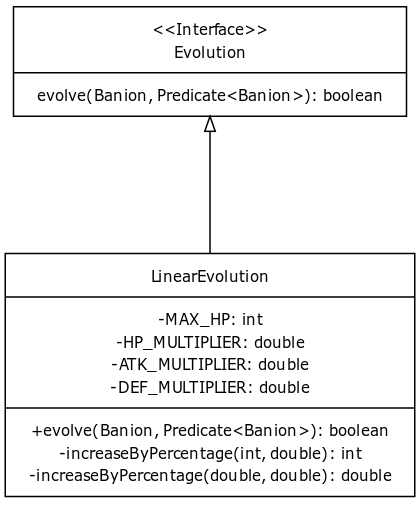
\includegraphics[scale=0.8]{evolution_uml}
    \end{figure}

    \subsubsection{\underline{Statistic}}
    \paragraph{Problem}
    The Banion's statistics need to be easily manipulated and have to accommodate different numerical data types to allow reusability.
    \paragraph{Solution}
    To encapsulate the representation of a statistic with a numerical primitive type (such as \verb|int|, \verb|double| and \verb|float|)
    a generic \verb|Statistic| interface was used.\\
    This interface generic type \verb|T| extends the abstract class \verb|Number|: this allows the use of primitive types to back a statistic object.\\
    A statistic is defined by a:

    \begin{itemize}
        \item \textbf{Type}: Attack, Defence, Hp;
        \item \textbf{Value}: the actual primitive value.
    \end{itemize}
    
    To unify these common characteristics an abstract class was used. The \verb|AbstractStatistic| constructor takes a \verb|String| to identify its type, and a
    \verb|T| for its value.\\
    Keeping a \verb|type| field is necessary to distinguish different statistics that may have the same numerical value, but differ in category.
    It was also deemed acceptable to use a \verb|String| for storing each statistic type since an abstract class cannot be instantiated and has to be extended by
    a concrete one, therefore keeping the \verb|String| creation inside the concrete constructor, and exposing only a \verb|T value| as its argument.

    \begin{lstlisting}[caption={Example of a concrete stat constructor.}, gobble=8]
        public ConcreteStat(final T value) {
            super("type", value);
        }
    \end{lstlisting}

    \begin{figure}[h]
    \centering{}
    \caption{Statistic UML diagram.}
    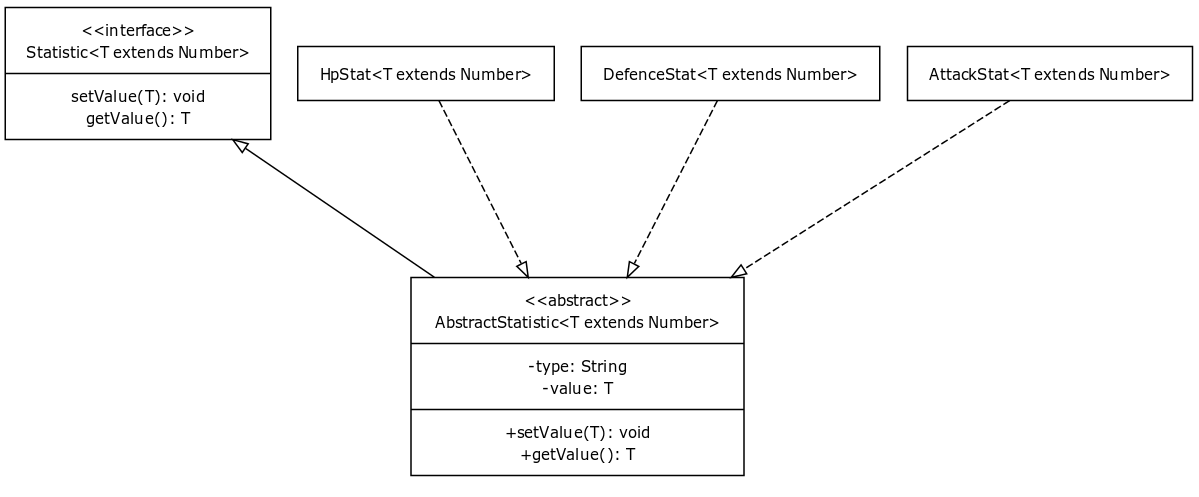
\includegraphics[width=\textwidth]{statistic_uml}
    \end{figure}

    \subsubsection{\underline{Die}}
    \paragraph{Problem}
    The player movement in the game board is determined by the roll of a die.
    \paragraph{Solution}
    The \verb|Die| class extends a specialization of an \verb|IntSupplier|, called \verb|PositiveIntSupplier|.
    This \verb|Die| represents a \href{https://en.wikipedia.org/wiki/Dice#Polyhedral_dice}{Polyhedral die}, meaning a
    three-dimensional die with polygonal faces, straight edges and sharp vertices.\\
    Polyhedral dice include the \textit{classic} cubical die, as well as non-cubical ones, such as tetrahedra, octahedra, dodecahedra
    and so on and so forth.\\
    There are many other rare variations of polyhedral dice, with various number of faces, but for the sake of simplicity
    a \verb|Die| instance was considered legal when its number of faces is even, and it is greater or equal to the minimum faces number.\\
    If this condition is not met, an \verb|IllegalArgumentException| will be thrown at construction.\\
    The \verb|Die| class internally uses a \verb|RandomGenerator| to generate pseudo-random sequences of integer values that represent
    the number drawn by the player.
    
    \begin{figure}[h]
    \centering{}
    \caption{Die UML diagram.}
    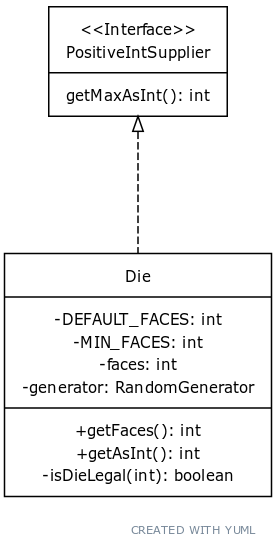
\includegraphics[scale=0.8]{die_uml}
    \end{figure}

    \subsubsection{\underline{SpriteAnimation}}
    \paragraph{Problem}
    Each Banion has an associated sprite sheet that has to be properly shown to the end user as an animated sprite.
    \paragraph{Solution}
    The class \verb|SpriteAnimation| was created to animate sprite sheets \cite{spriteSheets}. \verb|SpriteAnimation| \cite{spriteAnimation} extends JavaFX's Transition
    abstract class and was adapted for our intended use and needs.

    \begin{figure}[h]
    \centering{}
    \caption{The idle sprite sheet for \textbf{Infernhog}.}
    
\includegraphics[width=\textwidth]{spritesheet}
    \end{figure}

    This class \textit{slices} the sprite sheet into single sprites (given the dimensions of a single sprite) and sets the provided \verb|ImageView|'s viewport to said sprite.
    The aforementioned process is repeated for each individual sprite, creating the illusion of a single moving image for the player.\\
    A newer addition to the original \verb|SpriteAnimation| is the possibility to mirror the sprite horizontally. This enables the usage of
    the same sprite sheet for both the player and opponent's Banions, since they face each other in the battle GUI.\\
    Another new feature is the usage of an upscale multiplier for the sprite sheet image. To prevent the sprite to look too small
    and grainy a new \verb|Image| object with the requested dimensions (multiplied by the upscale factor), and the \verb|smooth| argument
    set to \verb|false| is created.
    This approach allows the sprites to be displayed crisply on screen.

    \subsubsection{\underline{GameSoundSystem}}
    \paragraph{Problem}
    The game needs a simple way to play background music and sounds effects.
    \paragraph{Solution}
    \verb|GameSoundSystem| is a helper class to play BGM\footnote{\textbf{BGM}: acronym for background music.} and SFX\footnote{\textbf{SFX}: acronym for sound effect.}.\\
    This audio playback helper class was conceived with these key components in mind:

    \begin{itemize}
        \item \textbf{Modularity} and \textbf{Encapsulation}: promotes modular design, code organization, easy maintenance and updating;
        \item \textbf{Reusability}: allows reusage across multiple classes without duplicating code;
        \item \textbf{Abstraction}: grants complex operations' encapsulation, reducing application complexity and ensuring efficient usage;
        \item \textbf{Extensibility}: enables the addition of new features, effects, and libraries without affecting other application components.
    \end{itemize}

    JavaFX's \textit{Media} module was used as the audio playback library. Different \verb|MediaPlayer|s were used to play BGM and SFX.
    This distinction allows the playback of both BGM and SFX simultaneously.\\
    Sounds will be loaded from their location into a \verb|Map| that links a \verb|String| containing the file name to a \verb|Pair| that contains the
    \verb|Media| object itself and an \verb|Optional<Duration>| that allows to trim the audio clip, if desired.\\
    The next paragraph will discuss the problems that were encountered while loading the audio resources from a JAR file.

    \subparagraph{Loading audio resources from JAR.}
    Loading audio resources at runtime from the jar file revealed itself to be a delicate matter: after an extensive research it was ascertained that loading
    sounds at runtime while running the application from an IDE/build tool and from the jar file required two different approaches. The latter required the use
    of the \verb|JarFile| class specified in the package \verb|java.util.jar|.\\
    To address this issue a solution \cite{jarFile} was found and incorporated after being properly adapted and refactored to follow our needs.\\
    Soundtracks by SketchyLogic \cite{bgm} were used for BGM, audio clips by OmegaPixelArt \cite{sfxGB} and ColorAlpha \cite{sfxMenu} were used for SFX.

    \subsection*{Raffaele Marrazzo}

    \dots

\chapter{Deployment}

\section{Automatized testing}

    We used \emph{JUnit} to test our \emph{Model} classes.

    Application components that underwent unit testing:

    \begin{itemize}
        \item Battle, Decision and Turn;
        \item AI;
        \item Difficulty;
        \item Evolution;
        \item Banion;
        \item Player \& Opponent;
        \item Moves;
        \item Die;
        \item Board;
        \item Engine;
        \item Banion deserialization.
    \end{itemize}

    The aforementioned components were regarded as key application's features, hence the decision of unit testing them.

\section{Work strategy}

    During development, we adopted the git-flow approach by creating a \verb|develop| branch and a new branch for each new \verb|feature|.

    We agreed upon the Model API interfaces, and we subsequently proceeded as follows:

    \subsection*{Enrico Marchionni}

    \begin{itemize}
        \item Engine and Board;
        \item Game difficulties;
        \item Entities generation;
        \item JavaFX \emph{View} controllers of start menu, login, difficulties selector, board, choose banions selector, and JavaFXView class;
        \item Main controller class.
    \end{itemize}

    \subsection*{Francesco Cipollone}

    \begin{itemize}
        \item GameEntity - Player \& Opponent;
        \item EntityController;
        \item Inventory;
        \item Evolution;
        \item Statistic;
        \item Die;
        \item SpriteAnimation;
        \item GameSoundSystem.
    \end{itemize}

    \subsection*{Raffaele Marrazzo}

    \dots

    \subsubsection*{Game components developed in conjunction}

    \begin{itemize}
        \item \verb|BattleView| and relative \verb|fxml|;
        \begin{itemize}
            \item Enrico Marchionni: sprites rendering;
            \item Francesco Cipollone: initialising a random background and music. Added SFX. Created the FXML;
            \item Raffaele Marrazzo: interaction with \verb|BattleController|, switch to Victory screen and Game Over screen.
        \end{itemize}
        \item \verb|ChooseBanionMenuView|;
        \begin{itemize}
            \item Enrico Marchionni: Event handlers, constructor;
            \item Raffaele Marrazzo: FXML.
        \end{itemize}
        \item \verb|BanionImpl|;
        \begin{itemize}
            \item Enrico Marchionni: the Banion implementation;
            \item Francesco Cipollone: included the evolution\label{multimap}.
        \end{itemize}
    \end{itemize}

\section{Development notes}

    Each one of us used these advanced aspects of the Java language:

    \subsection*{Enrico Marchionni}

        \subsubsection{Bounded type parameters}

        Used in a few occasions.

        Example at \url{https://github.com/DarwinsQuest/DarwinsQuest/blob/3ec97da07e9622ab8ec0333a774619be3332e88e/src/main/java/darwinsquest/util/EObserver.java#L15}.

        \subsubsection{Generic class}
        
        Used frequently.

        Example at \url{https://github.com/DarwinsQuest/DarwinsQuest/blob/3ec97da07e9622ab8ec0333a774619be3332e88e/src/main/java/darwinsquest/config/CustomDeserializer.java#L47}.

        \subsubsection{Annotation \emph{darwinsquest.annotation.Description}}

        I used this custom annotations in 2 different scopes.

        Example 1 at \url{https://github.com/DarwinsQuest/DarwinsQuest/blob/3ec97da07e9622ab8ec0333a774619be3332e88e/src/main/java/darwinsquest/core/EngineImpl.java#L38}.

        Example 2 at \url{https://github.com/DarwinsQuest/DarwinsQuest/blob/3ec97da07e9622ab8ec0333a774619be3332e88e/src/main/java/darwinsquest/view/JavaFXView.java#L56}.

        \subsubsection{Reflection}

        Used in different situations.

        Example at \url{https://github.com/DarwinsQuest/DarwinsQuest/blob/3ec97da07e9622ab8ec0333a774619be3332e88e/src/main/java/darwinsquest/core/EngineImpl.java#L65}.

        \subsubsection{Lambda expressions}

        Used very frequently.

        Example at \url{https://github.com/DarwinsQuest/DarwinsQuest/blob/3ec97da07e9622ab8ec0333a774619be3332e88e/src/main/java/darwinsquest/core/gameobject/banion/BanionImpl.java#L57}.

        \subsubsection{Optional}

        Used very frequently.

        Example at \url{https://github.com/DarwinsQuest/DarwinsQuest/blob/3ec97da07e9622ab8ec0333a774619be3332e88e/src/main/java/darwinsquest/core/Engine.java#L31}.

        \subsubsection{Stream}

        Used very frequently.

        Example at \url{https://github.com/DarwinsQuest/DarwinsQuest/blob/3ec97da07e9622ab8ec0333a774619be3332e88e/src/main/java/darwinsquest/view/ChooseBanionMenuView.java#L69}.

        \subsubsection{Immutable ordered set}

        Used only at \url{https://github.com/DarwinsQuest/DarwinsQuest/blob/3ec97da07e9622ab8ec0333a774619be3332e88e/src/main/java/darwinsquest/core/EngineImpl.java#L46}.

        \subsubsection{Library \href{https://openjfx.io/}{JavaFX}}
        
        Used for \emph{View} management.

        Example at \textit{fxml} with \textit{.css}, example at \url{https://github.com/DarwinsQuest/DarwinsQuest/blob/3ec97da07e9622ab8ec0333a774619be3332e88e/src/main/java/darwinsquest/view/JavaFXView.java#L53}.
        
        \subsubsection{Library \href{https://commons.apache.org/proper/commons-lang/}{Apache Commons Lang 3}}
        
        Used frequently.

        Example at \url{https://github.com/DarwinsQuest/DarwinsQuest/blob/3ec97da07e9622ab8ec0333a774619be3332e88e/src/main/java/darwinsquest/view/graphics/BanionsSpriteFactory.java#L27}.
        
        \subsubsection{Library \href{https://github.com/google/gson}{Google Gson}}
        
        Used for deserialization.

        Example at \url{https://github.com/DarwinsQuest/DarwinsQuest/blob/3ec97da07e9622ab8ec0333a774619be3332e88e/src/main/java/darwinsquest/util/JsonUtils.java#L81}.
        
        \subsubsection{Library \href{https://github.com/DiUS/java-faker}{Java Faker}}
        
        Used only at \url{https://github.com/DarwinsQuest/DarwinsQuest/blob/3ec97da07e9622ab8ec0333a774619be3332e88e/src/main/java/darwinsquest/core/difficulty/OpponentsFactoryImpl.java#L114}.

    \subsection*{Francesco Cipollone}

    \subsubsection{Use of \texttt{Optional}}
    Used in different occasions.\\
    Example at: \url{https://github.com/DarwinsQuest/DarwinsQuest/blob/64f84140f503f2e40d97e1dc69d0824c86c322e6/src/main/java/darwinsquest/core/gameobject/entity/AbstractGameEntity.java#L69-L75}

    \subsubsection{Generics}
    Used in the \verb|Statistic| interface and its subclasses.\\
    Example in \verb|AbstractStatistic|: \url{https://github.com/DarwinsQuest/DarwinsQuest/blob/64f84140f503f2e40d97e1dc69d0824c86c322e6/src/main/java/darwinsquest/core/statistic/AbstractStatistic.java#L9}

    \subsubsection{\texttt{Stream} and lambda expressions}
    Used in various sections.\\
    Example at: \url{https://github.com/DarwinsQuest/DarwinsQuest/blob/64f84140f503f2e40d97e1dc69d0824c86c322e6/src/main/java/darwinsquest/core/gameobject/entity/AbstractGameEntity.java#L61}

    \subsubsection{Creation of a \texttt{GameSoundSystem} with the JavaFX media module}
    Used in \verb|GameSoundSystem|.\\
    Example at: \url{https://github.com/DarwinsQuest/DarwinsQuest/blob/64f84140f503f2e40d97e1dc69d0824c86c322e6/src/main/java/darwinsquest/view/sound/GameSoundSystem.java#L30}

    \subsubsection{Use of \texttt{MultiValuedMap} from Apache Commons Collections 4}
    Used in \verb|Evolvable| interface, Look at \ref{multimap} for implementation details.\\
    Example at: \url{https://github.com/DarwinsQuest/DarwinsQuest/blob/64f84140f503f2e40d97e1dc69d0824c86c322e6/src/main/java/darwinsquest/core/evolution/Evolvable.java#LL11C29-L11C29}

    \subsection*{Raffaele Marrazzo}

    \dots

\chapter{Final comments}

    \paragraph{Tiles}
    Tile concept was never used in our battle \emph{Board} that consists in a series of battles that can be skipped by die jump.
    It would be better to introduce different \emph{Tile}s and to be forced to complete \emph{BattleTile}s, while the others can be skipped.

    \paragraph{AI}
    \dots

    \paragraph{Memory leak and profiling}
    During the late state of the project, a memory leak was discovered. This bug created serious performance issues, that caused the game to completely freeze
    during the battles.\\
    We, Francesco Cipollone and Raffaele Marrazzo, tried to perform a hot fix by using \textit{VisualVM} for profiling.
    The root of the problem was a faulty observers' management: each \verb|Observable| has a \verb|Collection| of observers that is always getting populated by
    new observers, but never freed of them, even when they are not needed anymore. This caused the \verb|Collection| to grow uncontrollably, leading to massive
    CPU and memory usage.\\
    For time concerns and the complexity (that was not debated during the course's lectures) of the problem, we were not able to fix it.\\
    To achieve acceptable performances during the game execution we decided to not alter the original architecture, but to decrease the possibility
    of a serious memory leak to happen by cutting the overall Banion's health points, making the battle shorter.

    \begin{figure}[H]
    \centering{}
    \caption{CPU and Memory usage snapshot}
    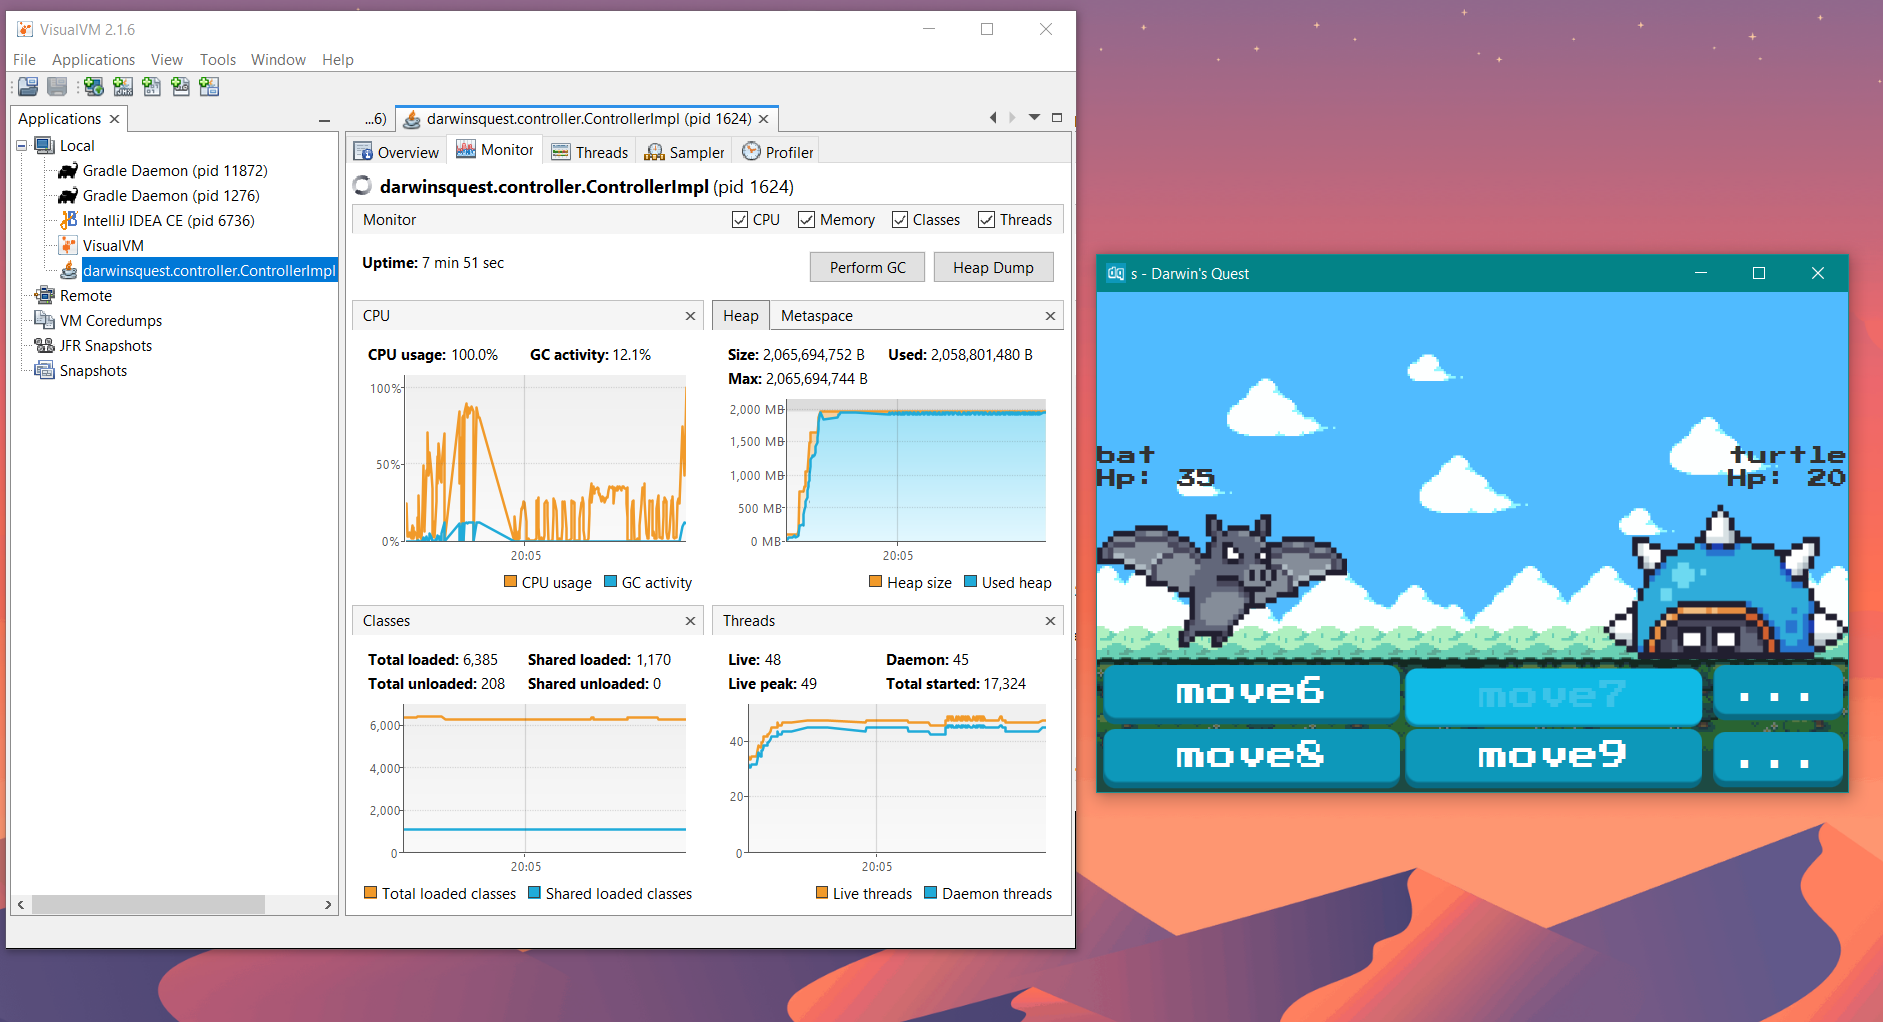
\includegraphics[width=\textwidth]{profiling1}
    \end{figure}

    \begin{figure}[H]
    \centering{}
    \caption{Memory sample snapshot}
    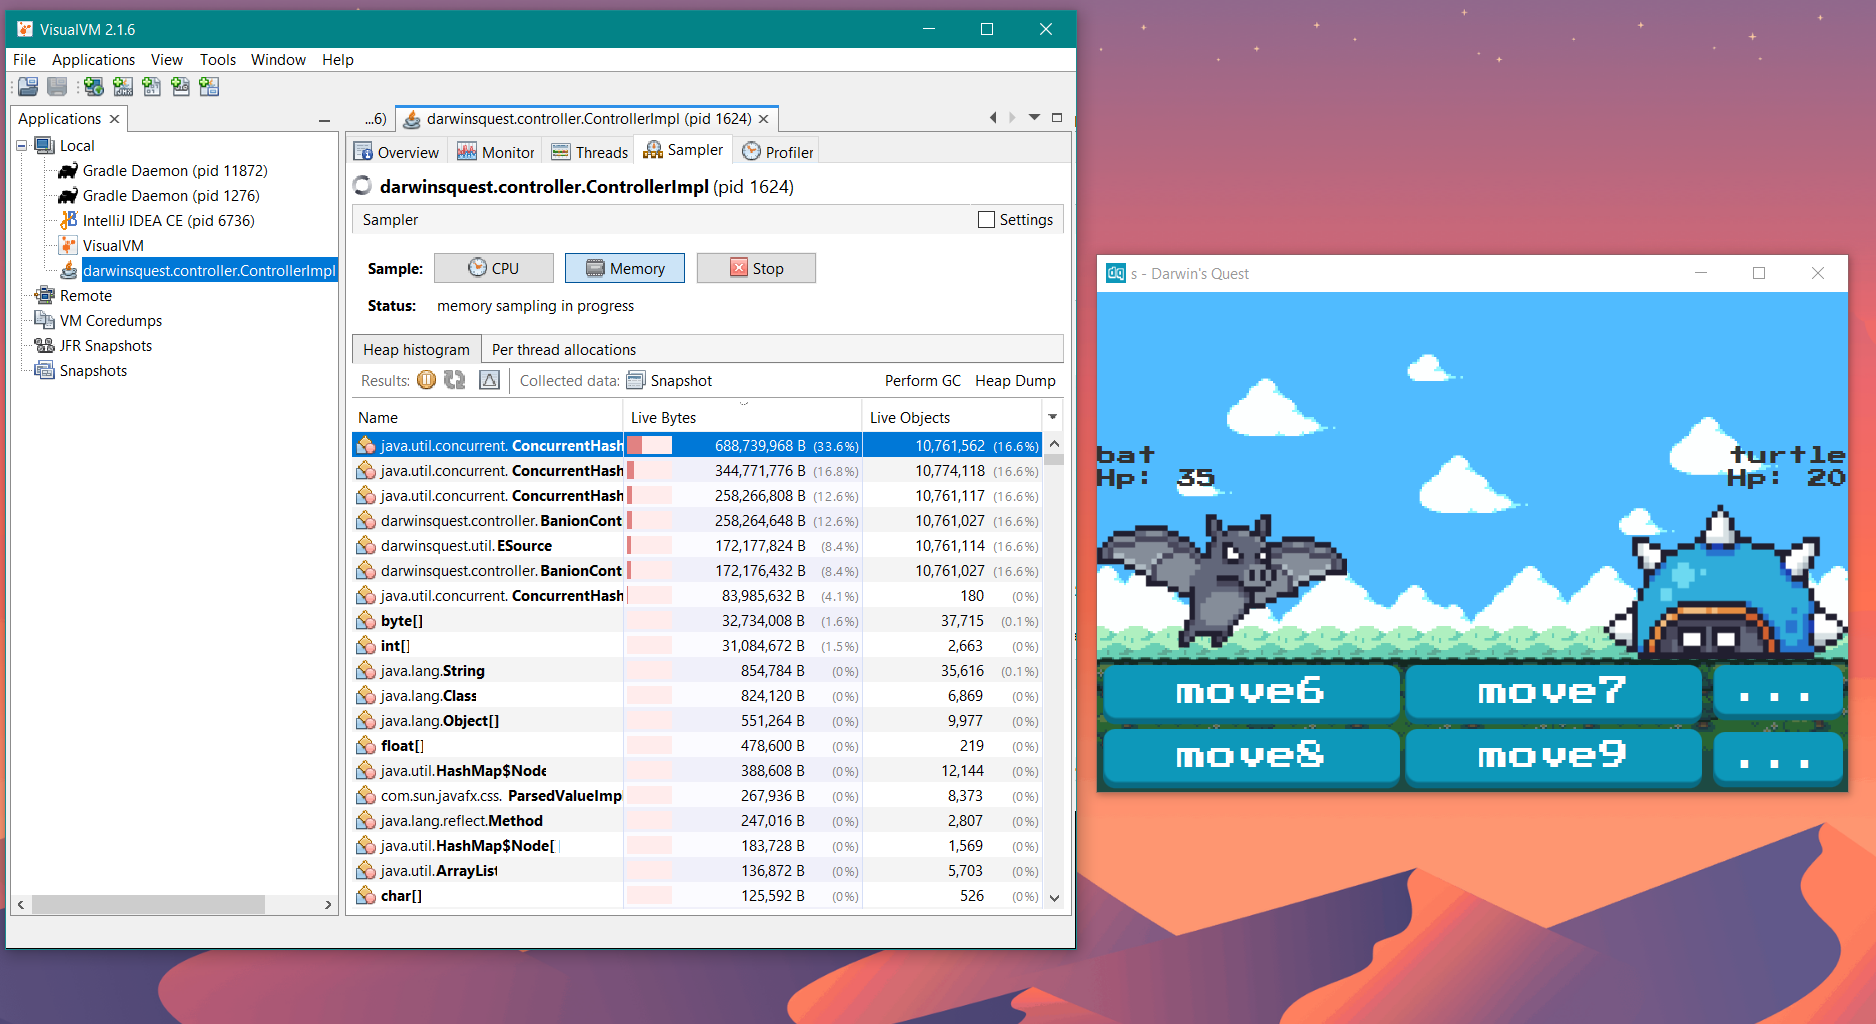
\includegraphics[width=\textwidth]{profiling2}
    \end{figure}

\section{Self-evaluation and future improvements}

    \subsection*{Francesco Cipollone}

    I am quite pleased on how this project turned out even if we did not manage to reach the level of complexity in game mechanics that we agreed upon.\\
    This was my first \textit{real} experience working with a small team of developers, and it strengthened my belief in how much important collaboration is.\\
    I have acquired a stronger sense of team effort, dedication and team management. I believe that the aforementioned skills are vital for teamwork and made
    me grow professionally.

    \subsection*{Raffaele Marrazzo}

    \dots

\section{Difficulties and comments to teachers}

    \subsection*{Francesco Cipollone}

    In contrast, I am thoroughly dissatisfied with how the interaction between certain team members in various circumstances was turbulent and unprofessional,
    frequently resulting in unproductive quarrels that only steered the project roadmap to the wrong direction, eventually resulting in low team morale.
    Poor communication frequently lead to commit wrong choices, and to partially inadequate priority judgement.\\
    There is a lot to ponder, and this experience will undoubtedly help us improve.

    \subsection*{Raffaele Marrazzo}

    I realised how fundamental time management is while working on this project: as beginners it was hard to evaluate in advance how much time we
    were going to invest on developing this game.\\
    To avoid getting ahead of ourselves, I feel that further instruction was required before confirming the project request.

\appendix

\chapter{User guide}

\section{Title Screen}
After running the game the user will be presented with a title screen with two buttons: ``Start'' and ``Quit''. To continue, the player should press the ``Start'' button.

\section{Username Selection}
After hitting ``Start'', the player will be asked to enter a username. Enter and confirm the appropriate username in the supplied input field.

\section{Banion Selection}
After confirming their username, the player will be taken to a menu where they can select four Banions for their team.
Select four Banions in the menu and then hit ``Confirm''.

\section{Game Difficulty Selection}
The player will be asked to select a game difficulty: ``Normal'' or ``Hard''. Select the desired level of difficulty by clicking on the corresponding option.

\section{Game board and Battles}
After selecting the game difficulty, the player will be taken to the game board screen. The game board represents the amount of battles to overcome before reaching the game's final boss.
Click the ``Fight'' button to begin a battle. Once a battle is won, press the ``Move'' button to progress further on the game board.

\section{Battle Mechanics}
During battles, the player will have several options available:
\begin{itemize}
  \item \textbf{Move Buttons}: These four buttons represent the available moves for the Banions in the player's inventory. Click on the desired move to execute it during the battle;
  \item \textbf{Swap Button}: This button allows the player to swap the active Banion with another one from their inventory. To swap the current Banion with the next one that is alive, click the Swap button;
  \item \textbf{End Button}: This button prematurely ends the battle, resulting in a loss.
\end{itemize}

\section{Additional Feature}
In every screen, except in battles, the player can access the ``Options'' menu by pressing the \verb|ESCAPE| key.
The ``Options'' menu allows the player to adjust the master volume. Click ``Close'' or press any button to return to the previous screen.\\
Dive into \emph{Darwin's Quest} and have a great time!


\chapter{Laboratory}

\section{enrico.marchionni@studio.unibo.it}

\begin{itemize}
    \item Lab 04: \url{https://virtuale.unibo.it/mod/forum/discuss.php?d=113869#p169173}
    \item Lab 05: \url{https://virtuale.unibo.it/mod/forum/discuss.php?d=114647#p169723}
    \item Lab 06: \url{https://virtuale.unibo.it/mod/forum/discuss.php?d=115548#p171159}
    \item Lab 07: \url{https://virtuale.unibo.it/mod/forum/discuss.php?d=117044#p173058}
    \item Lab 08: \url{https://virtuale.unibo.it/mod/forum/discuss.php?d=117852#p174127}
    \item Lab 09: \url{https://virtuale.unibo.it/mod/forum/discuss.php?d=118995#p175326}
    \item Lab 10: \url{https://virtuale.unibo.it/mod/forum/discuss.php?d=119938#p176522}
    \item Lab 11: \url{https://virtuale.unibo.it/mod/forum/discuss.php?d=121130#p177368}
    \item Lab 12: \url{https://virtuale.unibo.it/mod/forum/discuss.php?d=121885#p178425}
\end{itemize}

\section{francesco.cipollone@studio.unibo.it}

\begin{itemize}
    \item Lab 03: \url{https://virtuale.unibo.it/mod/forum/discuss.php?d=112846#p167954}
    \item Lab 04: \url{https://virtuale.unibo.it/mod/forum/discuss.php?d=113869#p169123}
    \item Lab 05: \url{https://virtuale.unibo.it/mod/forum/discuss.php?d=114647#p169538}
    \item Lab 06: \url{https://virtuale.unibo.it/mod/forum/discuss.php?d=115548#p171206}
    \item Lab 07: \url{https://virtuale.unibo.it/mod/forum/discuss.php?d=117044#p172980}
    \item Lab 08: \url{https://virtuale.unibo.it/mod/forum/discuss.php?d=117852#p174113}
    \item Lab 09: \url{https://virtuale.unibo.it/mod/forum/discuss.php?d=118995#p174912}
    \item Lab 10: \url{https://virtuale.unibo.it/mod/forum/discuss.php?d=119938#p176211}
    \item Lab 11: \url{https://virtuale.unibo.it/mod/forum/discuss.php?d=121130#p177361}
    \item Lab 12: \url{https://virtuale.unibo.it/mod/forum/discuss.php?d=121885#p178396}
\end{itemize}

\printbibliography

\end{document}